\section{基于增量舒尔补的优化方法}

iSAM2算法\cite{kaess2008isam,kaess2012isam2}创新性地在SLAM问题中使用了贝叶斯树来编码集束优化过程中的信息矩阵分解过程,达到高效地更新平方根信息矩阵的目的,显著地提升了全局优化的性能。其算法不仅适用于SLAM中的集束优化问题,也适用于一般的非线性最小二乘问题。也正是为了保证通用性,iSAM2难以在状态之间的关联特点高度统一的SLAM问题中发挥更高的性能。

例如在图\ref{fig:sparse_matrix}中,正规方程的三维点部分(左上角部分)高度稀疏,呈对角块状,在求解时应该优先考虑这一部分的分解。iSAM2算法需要依赖COLAMD\citep{davis2004algorithm}算法来被动地检测矩阵分解的顺序,一方面需要额外的计算时间,另一方面也不一定能得到比经验更好的结果。

\subsection{舒尔补}

\begin{figure}[htbp]
    \centering
    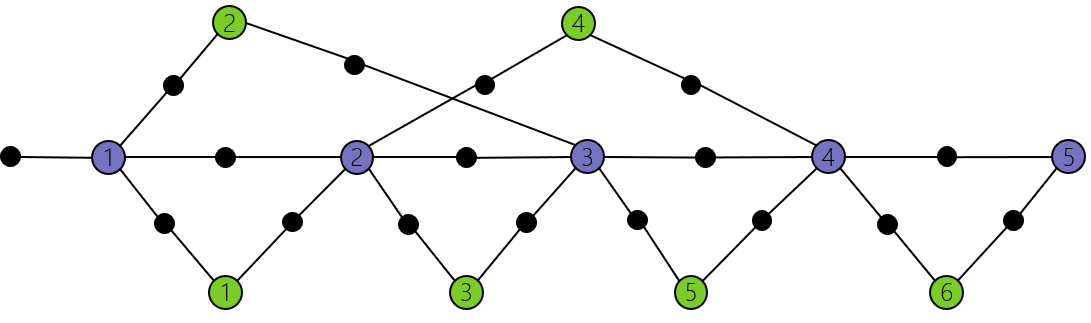
\includegraphics[width=\textwidth]{./figs/fg.png}
    \caption{因子图}
\end{figure}

\begin{figure}[htbp]
    \centering
    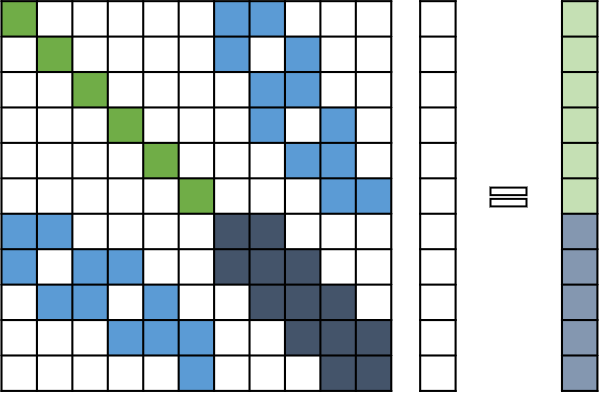
\includegraphics{./figs/normal_eq.png}
    \caption{正规方程}
\end{figure}

\begin{figure}[htbp]
    \centering
    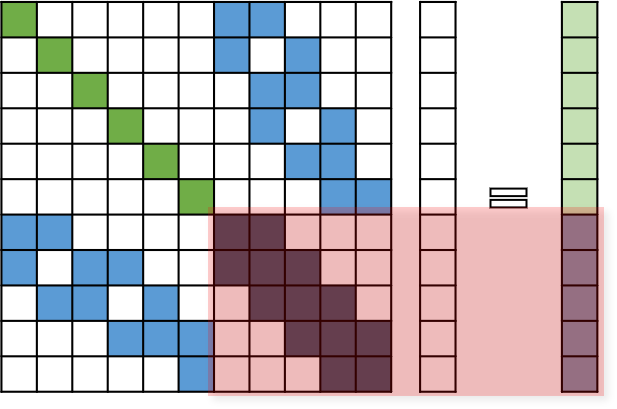
\includegraphics{./figs/reduced_sys.png}
    \caption{舒尔补}
\end{figure}

\begin{figure}[htbp]
    \centering
    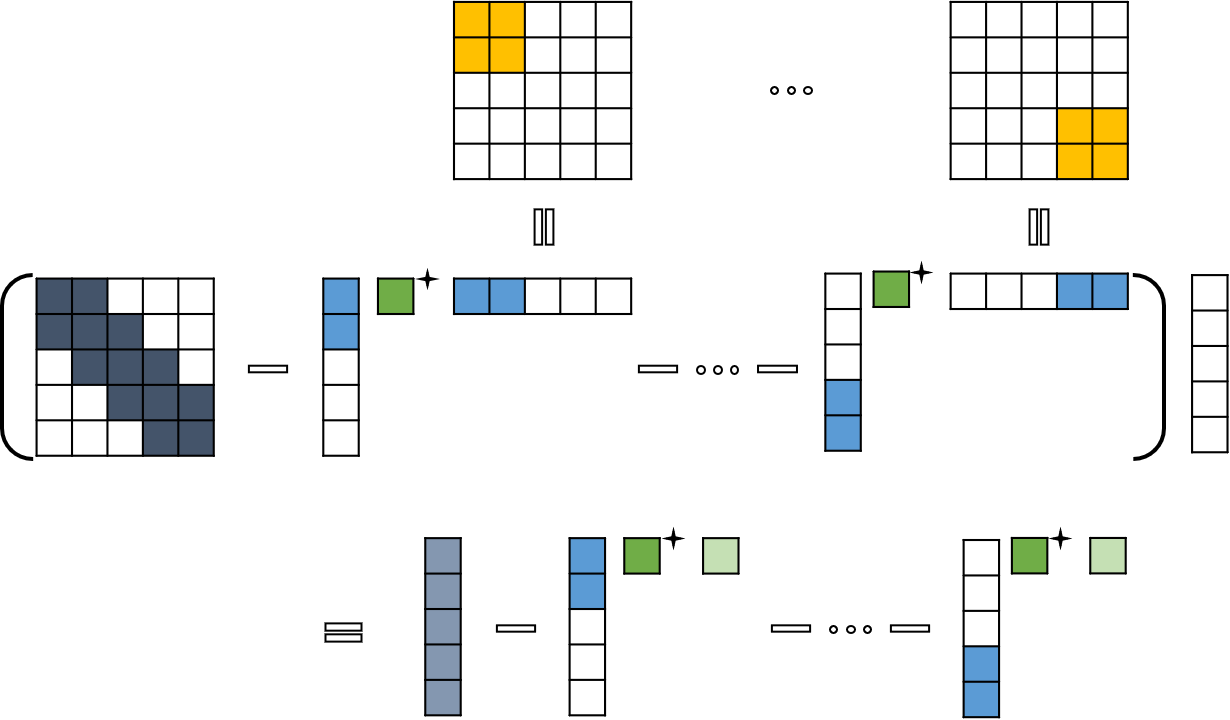
\includegraphics[width=\textwidth]{./figs/schur_complement.png}
    \caption{计算舒尔补}
\end{figure}

\subsection{增量更新舒尔补}

\begin{figure}[htbp]
    \centering
    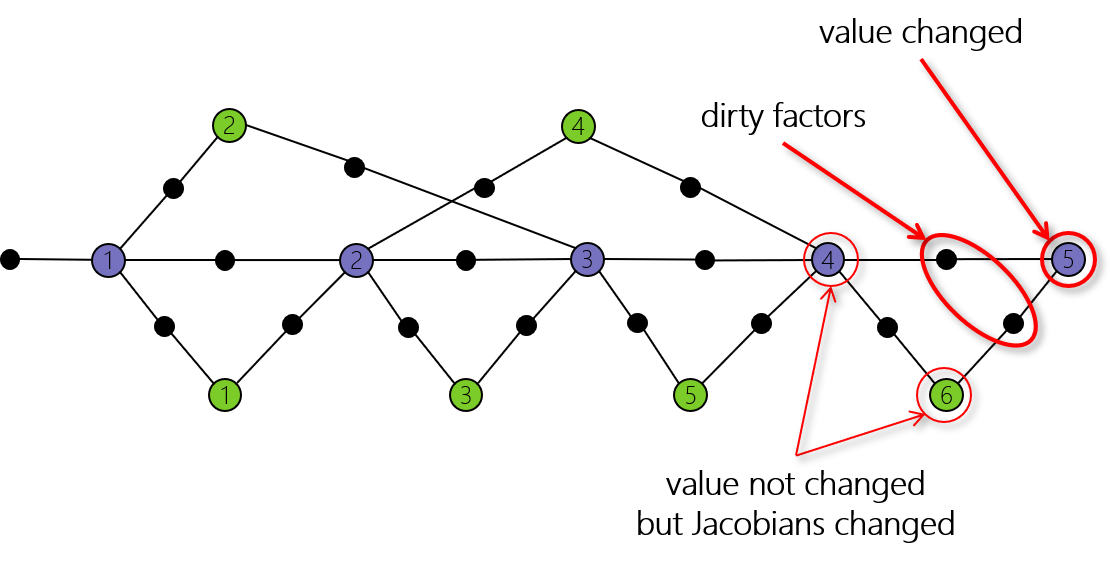
\includegraphics[width=\textwidth]{./figs/fg_cursed.png}
    \caption{标记因子图待更新部分}
\end{figure}

\begin{figure}[htbp]
    \centering
    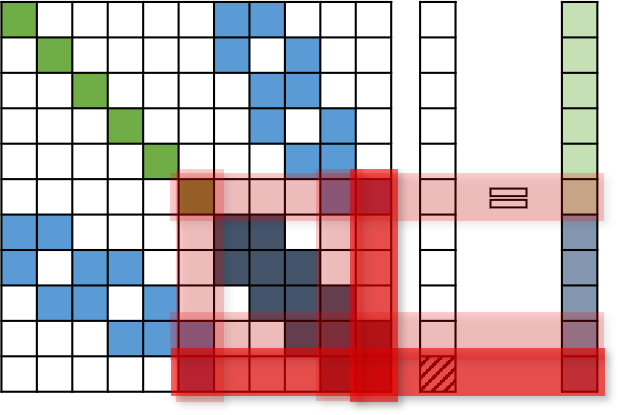
\includegraphics{./figs/normal_eq_cursed.png}
    \caption{待更新舒尔补部分}
\end{figure}

\begin{figure}[htbp]
    \centering
    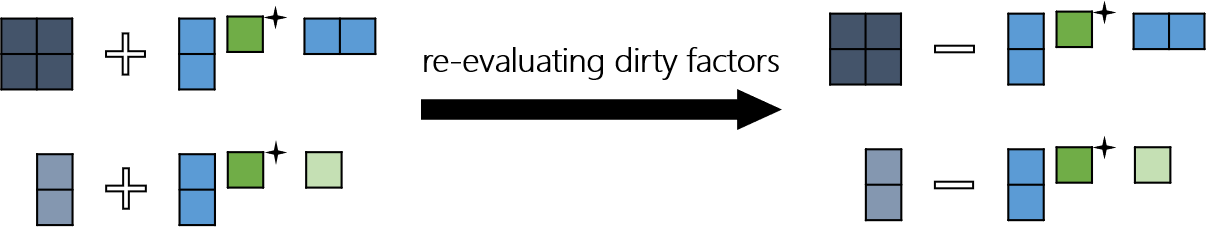
\includegraphics[width=\textwidth]{./figs/schur_update.png}
    \caption{更新舒尔补}
\end{figure}

\subsection{状态增广}

\begin{figure}[htbp]
    \centering
    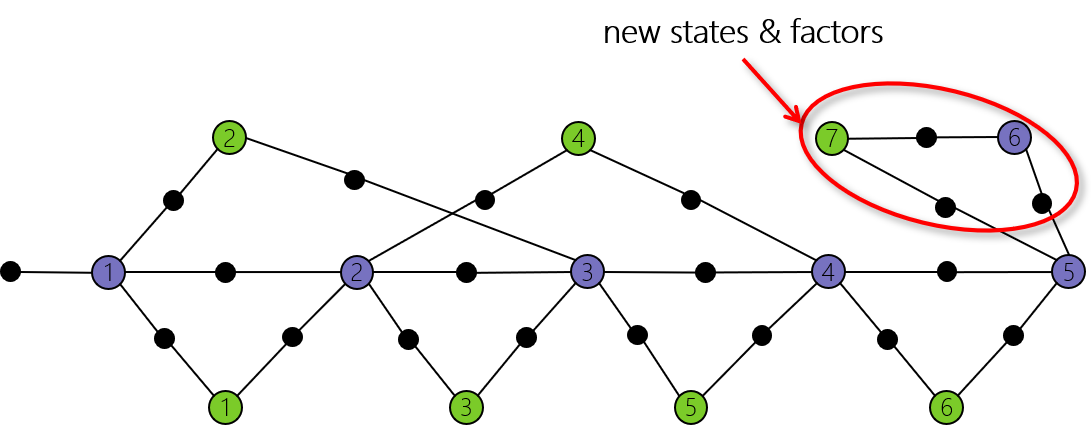
\includegraphics[width=\textwidth]{./figs/fg_aug.png}
    \caption{增广因子图}
\end{figure}

\begin{figure}[htbp]
    \centering
    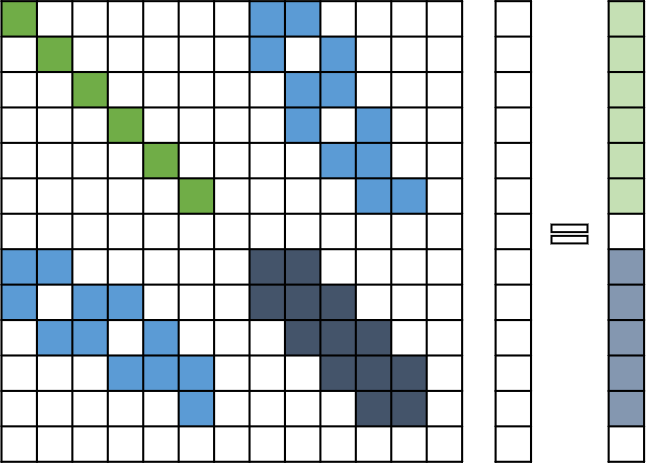
\includegraphics{./figs/normal_eq_aug.png}
    \caption{增广正规方程}
\end{figure}

\begin{figure}[htbp]
    \centering
    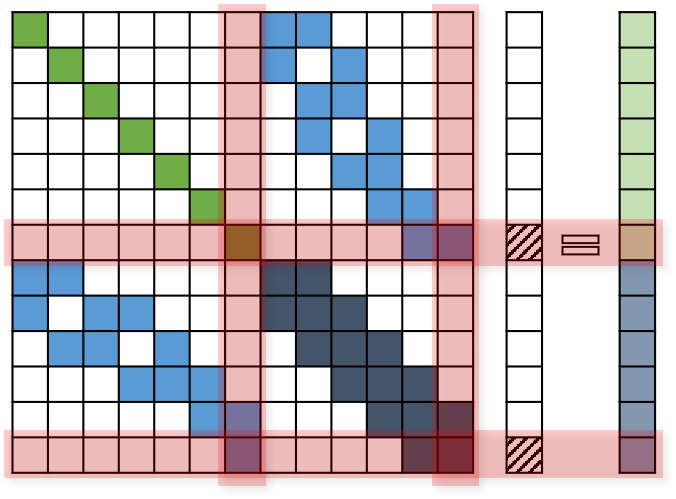
\includegraphics{./figs/normal_eq_update.png}
    \caption{更新正规方程}
\end{figure}

\subsection{增量舒尔补方法和基于贝叶斯树的增量方法对比}

\begin{figure}[htbp]
    \centering
    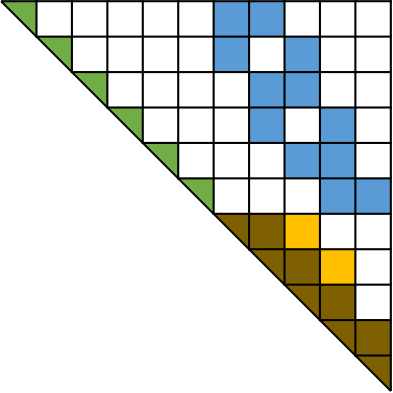
\includegraphics{./figs/sqrt_info.png}
    \caption{平方根信息矩阵}
\end{figure}

\begin{figure}[htbp]
    \centering
    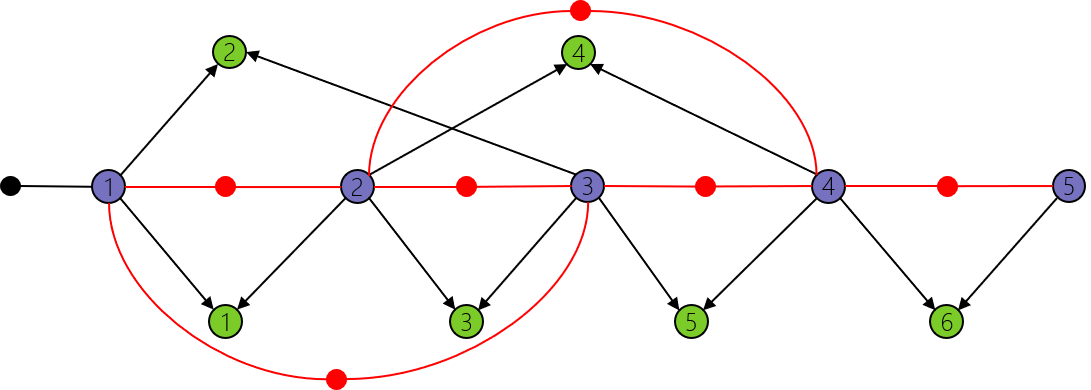
\includegraphics[width=\textwidth]{./figs/elim.png}
    \caption{消元}
\end{figure}

\begin{figure}[htbp]
    \centering
    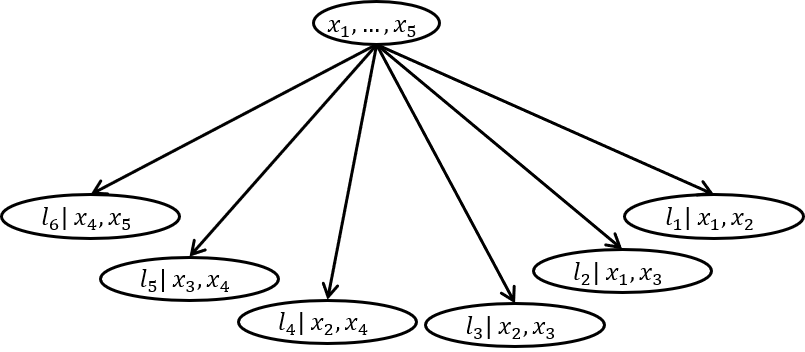
\includegraphics[width=\textwidth]{./figs/bayes_tree.png}
    \caption{贝叶斯树}
\end{figure}
